\section{Supplementary Notes}

\subsection{Pre-Transformation Module} \label{app:trans}
Let us review the process of computing the separability $\theta_{i,j}$. Given a feature pair $(f_i,f_j)$ and the corresponding positive and negative centroids, {\em (i)} we first compute $w_0$, $w_i$ and $w_j$ for $\lhat$\eat{ based on Equation~\ref{eqn:rep_line}}. Next, for each object $o_k$, {\em (ii)} we obtain the predicted label $\eta_{i,j}^{\lhat,k}$ according to Equation~\ref{eqn:est_label}. This step requires two multiplications and three additions. Finally, {\em (iii)} we calculate $\theta_{i,j}^{k}$ and the separability $\theta_{i,j}$ based on formulations in Section~\ref{sec:metric}\eat{Equation~\ref{eqn:s_object} and \ref{eqn:s_line} respectively}. This whole process is repeated for every feature pair candidate. However, there is massive redundancy across the processing of different feature pairs. For instance, when calculating the separability for two different feature pairs $(f_i,f_j)$ and $(f_i,f_{j'})$ with a common $f_i$, $w_i$ is in fact shared, and calculation of $w_i\cdot \mm_{i,k}$ in Equation~\ref{eqn:est_label} is repeated for each object $o_k$.
\tr{\sinha{is there another work we can cite that has done this?} \silu{Aditya's another paper~\cite{parameswaran2012crowdscreen} did similar trick, but in different problem. Do we want to cite it?}\agp{I think it's too far off.}}

Given this, we propose the \trans optimization module which will pre-calculate some common computational components once across different features and reuse these components the separability for each feature pair to eliminate the repeated computation. This \trans module transforms the original $\mm_{i,k}$ matrix into another space using our identified common feature pair components and updates the separability score equation accordingly.

For each feature $f_i$, we find the average values of the positive and negative objects for that feature, $\mm_i^+$ and $\mm_i^-$ respectively, and then we pre-transform $\mm_{i,k}$, i.e., the value of object $o_k$ on the feature $i$, to $\widehat{\mm}_{i,k}=$ $\Big( (\mm_i^+-\mm_i^-)\cdot \mm_{i,k}-\frac{(\mm_i^+)^2-(\mm_i^-)^2}{2} \Big) \cdot l_k$.
\eat{
\begin{equation}\label{eqn:matrix_transform}
\widehat{\mm}_{i,k} = \Big( (\mm_i^+-\mm_i^-)\cdot \mm_{i,k}-\frac{(\mm_i^+)^2-(\mm_i^-)^2}{2} \Big) \cdot l_k
\end{equation}
}
The basic idea is to decompose
Equation~\ref{eqn:est_label} into two components,
with each one only related to a single feature.
This transformation incorporates
the class centroids into the matrix values,
obviating their integration later
for every feature pair that involves the given feature.
We\eat{Equation~\ref{eqn:matrix_transform}} also multiplies
in the class label of the object, $l_k$,
rather than repeating this multiplication every time the object is evaluated (see example in Supplementary Figure~\ref{appF:transform}). With this transformation of the feature-object matrix,
evaluating whether an object was correctly separated is simplified as: if $sign(\widehat{\mm}_{i,k} + \widehat{\mm}_{j,k}) = 1$, then $\theta_{i,j}^{k}=1$; otherwise, $\theta_{i,j}^{k}=0$. \eat{from Equation~\ref{eqn:s_object} into Equation~\ref{eqn:s_object_transform}:

\begin{equation}\label{eqn:s_object_transform}
\theta_{i,j}^{k}=\left\{
 \begin{array}{ll}
  1 \textit{\hspace{2mm} if \hspace{2mm}} sign(\widehat{\mm}_{i,k} + \widehat{\mm}_{j,k}) = 1\\
  0 \textit{\hspace{2mm} otherwise \hspace{2mm}}
 \end{array}
 \right.
\end{equation}

After pre-transformation, we are now ready
to compute the separability score $\theta_{i,j}$.
Given a feature pair $(f_i,f_j)$, we can compute $\theta_{i,j}^{k}$
for each object $o_k$ based on Equation~\ref{eqn:s_object_transform}.}
Note that this step only involves one addition and one comparison and is performed only once for each feature.
Next, we can calculate overall separability score $\theta_{i,j} = \sum_{k}{\theta_{i,j}^{k}}$\eat{ like in Equation~\ref{eqn:s_line} without the pre-transformation}. Overall,
we not only eliminate the steps of computing
$w_0$, $w_i$ and $w_j$ for every feature pair,
but also reduce the cost of calculating
$\eta_{i,j}^{k}$ in Equation~\ref{eqn:est_label}.
With the \trans module, we calculate $\widehat{\mm}$ as a pre-transformation step,
and use it when evaluating feature pairs instead of $\mm$ and calculate $\theta_{i,j}$ accordingly\eat{
and Equation~\ref{eqn:s_object_transform} instead of
Equation~\ref{eqn:est_label} and~\ref{eqn:s_object}}.


\subsection{Estimation Accuracy in \sampling Module} \label{app:sampling}
We have proposed \sampling for estimating $\theta_{i,j}$ in Section~\ref{ssec:sampling}. Next, we formally quantize the sample set size in Theorem~\ref{them:est}.

\begin{theorem}[Estimation Accuracy]\label{them:est}
By considering $\Omega(\frac{1}{\epsilon^2}\cdot \log(\frac{1}{\delta}))$ samples, with probability at least $1-\delta$, we have $|\frac{\theta_{i,j}(\sss)}{|\sss|}-\frac{\theta_{i,j}}{n}| \leq \epsilon$, i.e., $|\tilde{\theta}_{i,j}-\theta_{i,j}|\leq \epsilon n$.
\end{theorem}
\tr{\begin{proof}
  Based on Hoeffding's inequality:
  $$Pr(|\frac{\theta_{i,j}(\sss)}{|\sss|}-\frac{\theta_{i,j}}{n}| \geq \epsilon) \leq 2e^{-2|\sss|\epsilon^2}$$
  Hence, when $|\sss| = \frac{1}{2\epsilon^2}\cdot \log(\frac{2}{\delta}) = \Omega(\frac{1}{\epsilon^2}\cdot \log(\frac{1}{\delta}))$, we have:
$$
  Pr(|\frac{\theta_{i,j}(\sss)}{|\sss|}-\frac{\theta_{i,j}}{n}| \geq \fepsilon) \leq \delta \ \ \ \ \ \ \ \ \ \ \ \square
$$
\end{proof}
}
\noindent We can treat $\log(1/\delta)$ as a constant, e.g., by setting $\delta = 0.05$. Thus, Theorem~\ref{them:est} essentially states that with only $\Omega(\frac{1}{\epsilon^2})$ samples, with probability 95\%, the confidence interval for $\theta_{i,j}$ is $[\tilde{\theta}_{i,j}-\epsilon n, \tilde{\theta}_{i,j}+\epsilon n]$.


\subsection{Construction of \msig Feature-Object Matrix} \label{app:msig_matrix}
To construct the feature-object matrix for \msig, which has gene objects and gene property features, we collected prior knowledge about gene annotations and protein homology from several databases.
Our gene annotations and gene properties were extracted from Gene Ontology terms~\cite{gene2014gene},
PFam domains~\cite{finn2015pfam}, and Reactome~\cite{fabregat2017reactome}  and KEGG~\cite{kanehisa2016kegg} pathways.
We constructed a heterogeneous  network with nodes for all 22,210 genes and 21,235 properties from these databases and with edges representing their annotations between genes and properties.
We also created weighted homology-based edges in the network between pairs of genes based on their protein sequence similarity as determined by BLAST scores~\cite{altschul1990basic}.
We used the first phase of the DRaWR algorithm~\cite{blatti2016characterizing} with a restart probability of 0.5 to perform a random walk restarting from each gene node on the heterogeneous network, thereby scoring the connectivity of all nodes in the network to the gene.
For each gene-property pair ($g$, $r$), we assigned the numeric value from the random walk stationary probability distribution that represents not only whether the gene is annotated with that property, but also whether other genes closely related to gene $g$ are annotated with property $r$.
We thus obtained a feature-object matrix describing each gene (object) as a vector of its strength of association with each property (feature) in light of prior biological knowledge.


\subsection{Speedup Analysis for \lincs} \label{app:lincs}
In Figure~\ref{fig:lincs_time}, we observe over $400\times$ average decrease in the running time of finding the \topk feature pairs that separate the \lincs experiments of a single perturbagen from others. The greatest speedup comes with adding the \sampling module, where only $100K$ feature pair candidates, i.e., $|\cc|$, are checked out of all $250M$ feature pairs (Supplementary Table~\ref{appT:time}). For the selected algorithms with best running times, \horiz and \vertic, the pre-transformation and feature ordering overhead account for an average of $45+35=80s$ of the overall 104 and 94 median seconds respectively.


\subsection{Gene Interaction Datasets} \label{app:relation_data}
For our knowledge bases of protein and gene interactions, we downloaded datasets derived from 8 data sources:
STRING~\cite{szklarczyk2014string}, Reactome~\cite{croft2013reactome}, Pathway Commons~\cite{cerami2010pathway},
HumanNet~\cite{lee2011prioritizing}, BioGRID~\cite{chatr2017biogrid}, Intact~\cite{orchard2013mintact},
DIP~\cite{salwinski2004database}, and BLAST~\cite{altschul1990basic} databases. 
The datasets were downloaded, harmonized, and mapped to Ensembl gene identifiers using the 
KnowEnG Knowledge Network Builder \url{https://github.com/KnowEnG/KN_Builder}. 
The final processed network used in this work can be downloaded from \url{https://github.com/KnowEnG/KN_Fetcher/blob/master/Contents.md#gene}.


\section{Supplementary Tables}

\subsection{\genviz Method Notation}\label{appT:notation}
Notation used in this paper.
\begin{table}[h]
\centering
\vspace{-1mm}
\small
\begin{tabular}{|c|c|c|c|}
 \hline
 Symb. & Description & Symb. & Description\\
 \hline
 \hline
 $\mm$ & feature-object matrix & $\ff$ & feature set in $\mm$ \\
 \hline
 $f_i$ & feature $i$ in $\ff$ & $m$ & number of features in $\ff$\\
 \hline
 $\oo$ & object set in $\mm$ & $N$ & number of objects in $\oo$\\
 \hline
 $\oo_+$ & positive object set & $\oo_-$ & negative object set\\
 \hline
 $\widehat{\oo}$ & labelled object set & $n$ & number of labelled objects in $\widehat{\oo}$\\
 \hline
 $o_k$ & object $k$ in $\widehat{\oo}$ & $l_k$ & label of object $o_k$\\
 \hline
 $\ell$ & separating line in 2-D & $\lhat$ & representative line in 2-D\\
 \hline
 $\eta_{i,j}^{\ell,k}$ & predicted label of $o_k$ & $\theta_{i,j}^{\ell,k}$ & $o_k$ is correctly separated? \\
 \hline
 $\theta_{i,j}^{\ell}$ & \# correctly separated $o_k$ & $\theta_{i,j}$ & separability score\\
 \hline
 $\widehat{\mm}$ & $\mm$ after transformation & $\tilde{\theta}_{i,j}$ & estimated $\theta_{i,j}$\\
 \hline
 \end{tabular}
%\caption{\scriptsize Notation used in this paper.}
\label{tbl:notation}
\vspace{-8pt}
\end{table}

%\subsection{Time Complexity of Selected Algorithms}\label{appT:time}
%Time Complexity of the Selected Algorithms. Here, $m$ and $n$ are the number of features and objects, $\sss$ is the sampled set size, $\chi$ is the limit on the number of feature pairs considered, and $\cc$ is the number of generated feature pair candidates.
%\begin{table}[h]
%\centering
%\vspace{-5mm}
%\small
%\begin{tabular}{|c||c|}
 %\hline
% \hline
% & Complexity\\
% \hline
% \baseline &$O(m^2n)$\\
% \hline
% %\early & yes & yes & no & no & no & Any & no & $O(m^2n)$\\
% % \hline
% \earlyOrder  & $O(m^2n)$\\
% \hline
% \samp   & $O(mn+m^2|\sss|+|\cc|n)$\\
% \hline
% \sampOpt  & $O(mn+m^2|\sss|+|\cc|n)$\\
% \hline
% \horiz   & $O(mn+\chi|\sss|+|\cc|n)$\\
% \hline
% \vertic  & $O(mn+\chi|\sss|+|\cc|n)$ \\
% \hline
% \end{tabular}
%\caption{Time Complexity of the Selected Algorithms. Here, $m$ and $n$ are the number of features and objects, $\sss$ is the sampled set size, $\chi$ is the limit on the number of feature pairs considered, and $\cc$ is the number of generated feature pair candidates.}
%\label{tbl:alg_time}
%\end{table}

\subsection{Running Time Detailed Comparison}\label{appT:time}
For each dataset collection, MSigDB and LINCS, show two statistics FPsChecked and ObjectsChecked, for each optimization module phase (columns).  FPsChecked is the number of feature pairs evaluated in the phase, and ObjectsChecked is the average number of sample objects that are evaluated across all feature pairs.

\subsection{In-depth Analysis of 'Improved' Feature Pairs}\label{appT:fp}
For each drug dataset (col C), we return a limited number of gene feature pairs (cols E,F) that after correction were the most "improved" over their corresponding single feature results either by the change in the corrected\_pvalue (cols H,I,J,N,O) or the change in the feature rankings (cols K,L,M,P).  Pubmed IDs (cols Q,R) are provided when the relationship between the drug and the gene feature were found in the Comparative Toxicogenomics Database (CTD) or by manual literature search (denoted by *-asterisk).  When relationships between the gene features themselves were discovered, the type and strength of the relationships were reported (col S) and the number of relationships quantified (col T).


\section{Supplementary Figures}

\subsection{Example for \trans Module}\label{appF:transform}
The \trans module is applied once to the original values in the feature-object matrix $\mm$ (above) to produce $\widehat{\mm}$ (below). For two features, $f_i$ and $f_j$. The top half depicts $\mm_{i,k}$ and $\mm_{j,k}$ before transformation, where green color represents a positive label and red color represents a negative label. In this example, the centroids of the positive and negative objects are $\mu_{i,j}^+=(5,7)$ and $\mu_{i,j}^-=(3,5)$ respectively. Hence, we can rewrite $\widehat{\mm}_{i,k} = (2\mm_{i,k}-8)\cdot l_k$ and $\widehat{\mm}_{j,k} = (2\mm_{i,k}-12)\cdot l_k$ for features $f_i$ and $f_j$ respectively. After calculation, we can obtain the values for $\widehat{\mm}_{i,k}$ and $\widehat{\mm}_{j,k}$ shown in the bottom half.
\begin{figure}[!htb]
\centering %%% not \center
\vspace{-5mm}
\includegraphics[width=.4\textwidth]{fig/transformation.eps}
%\vspace{-5mm}
%\caption{The \trans module is applied once to the original values in the feature-object matrix $\mm$ (above) to produce $\widehat{\mm}$ (below). For two features, $f_i$ and $f_j$. The top half depicts $\mm_{i,k}$ and $\mm_{j,k}$ before transformation, where green color represents a positive label and red color represents a negative label. In this example, the centroids of the positive and negative objects are $\mu_{i,j}^+=(5,7)$ and $\mu_{i,j}^-=(3,5)$ respectively. Hence, we can rewrite $\widehat{\mm}_{i,k} = (2\mm_{i,k}-8)\cdot l_k$ and $\widehat{\mm}_{j,k} = (2\mm_{i,k}-12)\cdot l_k$ for features $f_i$ and $f_j$ respectively. After calculation, we can obtain the values for $\widehat{\mm}_{i,k}$ and $\widehat{\mm}_{j,k}$ shown in the bottom half.}
\vspace{-8mm}
\label{fig:trans_term}
\end{figure}


\subsection{Illustration for \traversal Module}\label{appF:traversal}
We rank individual features based on their single feature separability scores, $\theta_{i,i}$, from best to worst, $\{f_1^{'} f_2^{'},\cdots,f_m^{'}\}$.
\begin{itemize}
 \item \emph{Horizontal traversal:} For each feature $f_i^{'}$, pair it with each other feature $f_j^{'}$, where $j \geq i$, to obtain $(f_i^{'},f_j^{'})$. Repeat for each $f_i^{'}$, where $1 \leq i\leq m$.
 \item \emph{Vertical traversal:} For each feature $f_j^{'}$, pair it with each other feature $f_i^{'}$, where $i \leq j$, to obtain $(f_i^{'},f_j^{'})$. Repeat for each $f_j^{'}$, where $1 \leq j\leq m$.
\end{itemize}

\begin{figure}[!htb]
 \centering
 \vspace{-5mm}
 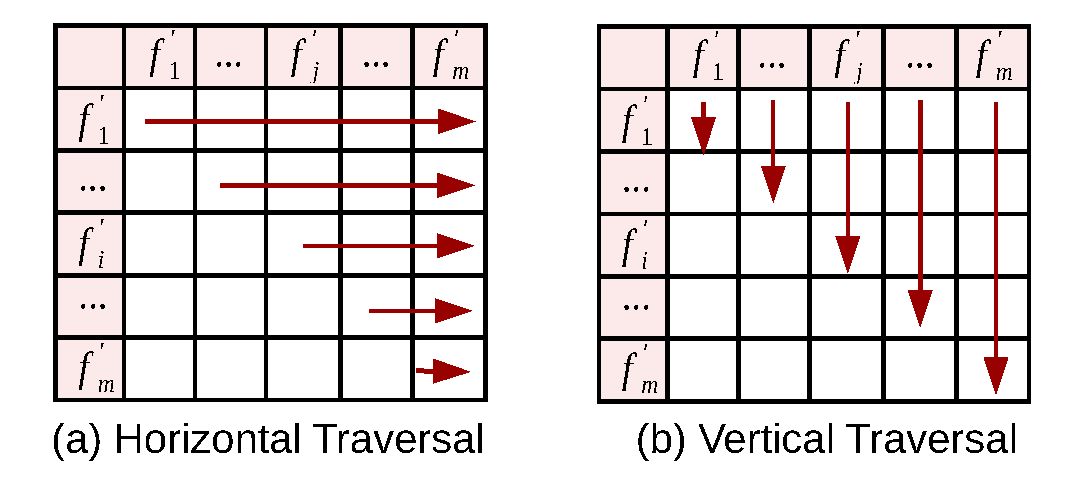
\includegraphics[width=0.7\linewidth]{fig/traversal.eps}
% \vspace{-5mm}
%\caption{After feature ordering, \traversal enables \genviz is able to examine the feature pair search space (a) horizontally or (b) vertically.}
\vspace{-5mm}
\label{fig:traversal}
\end{figure}

For an example, suppose there are 20,000 features, $m=2\times 10^4$. Initially, the number of possible feature pairs is roughly $\frac{m^2}{2}=2\times 10^8$. However, if we limit the number of considered feature pairs to $\chi=10^7$, we reduce our search space to $\frac{1}{20}$ of the total number of feature pairs. We order the single features by their individual separability scores. In horizontal traversal, only feature pairs with at least one individual feature ranked in the top 500 will be considered; while vertical traversal will consider only feature pairs with both individual features ranked better than 2000.


\subsection{Separability Score Comparison}~\label{appF:exp_sep}
Comparison of Brute Force-based and Rocchio-based separability score. (a) For each of 10 datasets, we display the ratio of the true separability score between the best feature pair chosen by brute force and by the Rocchio-based method. (b) For each dataset, we display the ratio of the true separability score and the Rocchio-based separability score for the best feature pair selected using Rocchio-based method.
\begin{figure}[!htb]
\centering %%% not \center
\vspace{-5mm}
\subfigure[Best Feature Pair Comparison]{\label{fig:brute_rocchio_ratio}\includegraphics[width=.4\textwidth]{fig/rocchio_brute_ratio.eps}}
\subfigure[Measure Comparison]{\label{fig:brute_rocchio_score}\includegraphics[width=.4\textwidth]{fig/rocchio_brute_score.eps}}
%\vspace{-5mm}
%\caption{Comparison of Brute Force-based and Rocchio-based separability score. (a) For each of 10 datasets, we display the ratio of the true separability score between the best feature pair chosen by brute force and by the Rocchio-based method. (b) For each dataset, we display the ratio of the true separability score and the Rocchio-based separability score for the best feature pair selected using Rocchio-based method.}
\vspace{-5mm}
\label{fig:brute_rocchio}
\end{figure}


\subsection{Histogram of $improv\_quot$}~\label{appF_exp_hist}
Histogram of $improv\_quot$. For the \toptwenty feature pairs from all runs from the (a) \msig and (b) \lincs datasets, distribution of the improvement of the feature pair significance over the corresponding single feature significance. The red line shows the significance threshold of 5.
\begin{figure}[!htb]
\centering %%% not \center
\vspace{-5mm}
\subfigure[\msig]{\label{fig:msig_histogram_diff}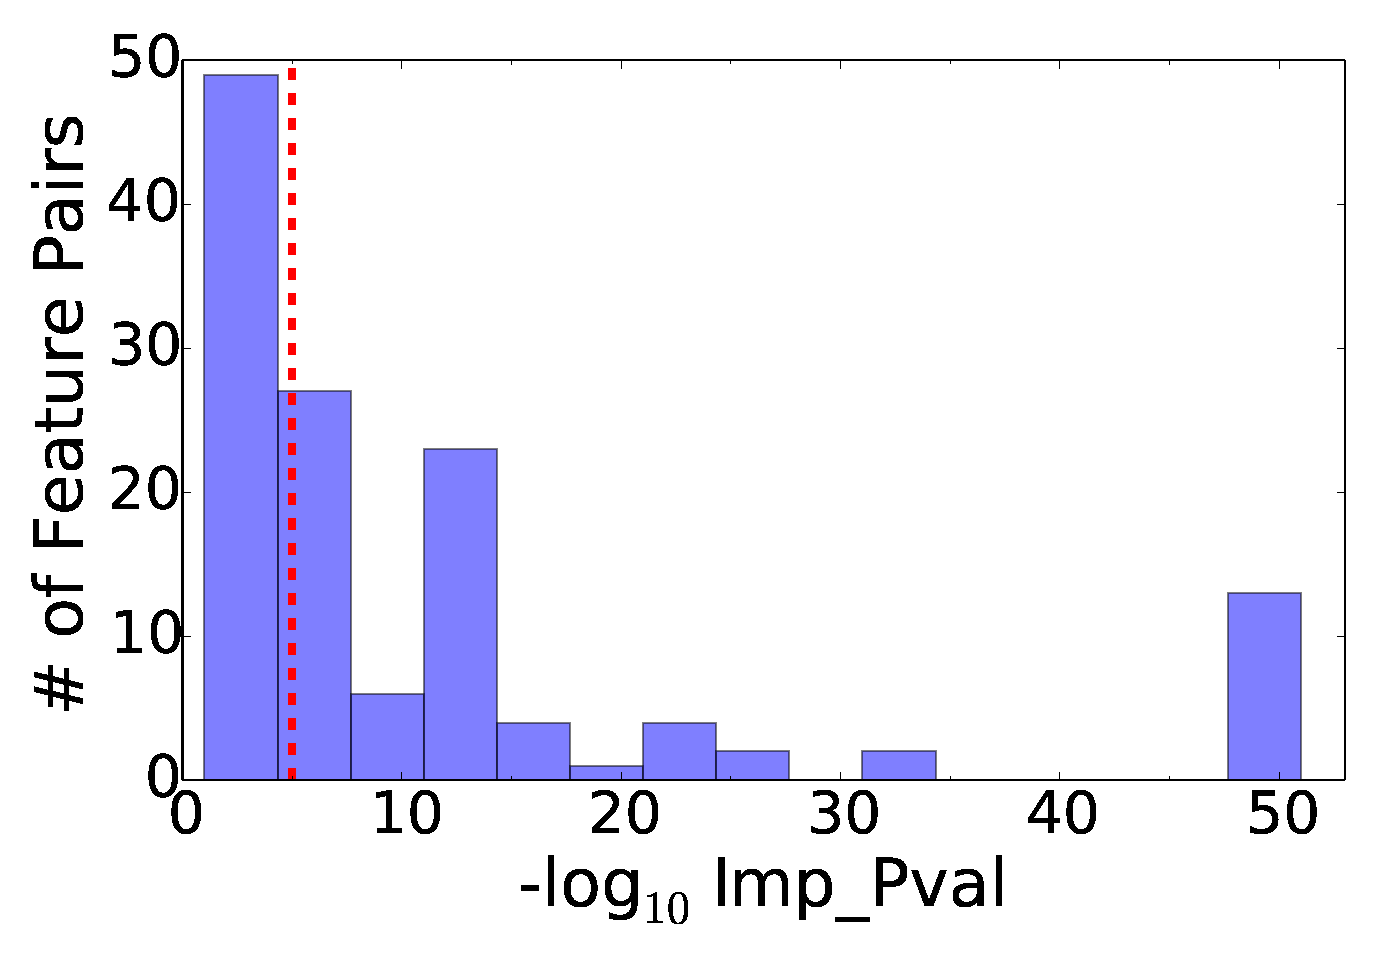
\includegraphics[width=.4\textwidth]{fig/histogram_msig_diff_pval.eps}}
\subfigure[\lincs]{\label{fig:lincs_histogram_diff}\includegraphics[width=.4\textwidth]{fig/histogram_lincs_diff_pval.eps}}
%\vspace{-5mm}
%\caption{Histogram of $improv\_quot$. For the \toptwenty feature pairs from all runs from the (a) \msig and (b) \lincs datasets, distribution of the improvement of the feature pair significance over the corresponding single feature significance. The red line shows the significance threshold of 5.}
\vspace{-3mm}
\label{fig:histogram_diff}
\end{figure}
